\documentclass[11pt]{report}
\usepackage{fancyhdr}
\usepackage{fancybox}
\usepackage{tipa}
\usepackage{framed}
\usepackage[retainorgcmds]{IEEEtrantools}
\usepackage[utf8x]{inputenc}
\usepackage{epsfig}
\usepackage{anysize}
\usepackage{gensymb}
\usepackage{amssymb}
\usepackage{graphicx}
%\usepackage[demo]{graphicx}
\usepackage{caption}
\usepackage{subcaption}
\usepackage[utf8x]{inputenc}
\usepackage{longtable}
\usepackage{url}
\usepackage{plain}
\usepackage{mathtools}
%\renewcommand{\bibname}{References}
%\usepackage{hyperref}
\usepackage[plainpages=false]{hyperref}
\hypersetup{
    colorlinks=true,
    linkcolor=black,
    citecolor=black,
    filecolor=black,
    urlcolor=black,
}
\lhead{}


\setcounter{page}{-100}
\setcounter{secnumdepth}{5}

\newenvironment{fminipage}%
{\begin{Sbox}\begin{minipage}}%
{\end{minipage}\end{Sbox}\fbox{\TheSbox}}
% Title Page
\title{\textbf{Checking Information Misuse in DroidRacer Traces using RWFM Model}}
\vspace{2.5cm}
\author{\bf{A R\&D Report}\\
        \\
        \emph{Submitted in partial fulfillment of requirements for degree of}\\
        \\
        \bf{Masters of Technology}\\
        \\
        \emph{by}\\
        \\
		\bf{Asif Ali}\\
        \bf{Roll No : 143059009}\\
        \\
        \emph{under the guidance of}\\
        \\
        \bf{Prof. R.K. Shyamasundar}\\
        \\\\
        
\includegraphics[height=3.5cm]{./images/iitb_logo}\\
        \\
        \bf{Department of Computer Science and Engineering}\\
        \bf{Indian Institute of Technology, Bombay}\\
}
\date{May, 2016}


% page layout settings

% \setlength{\parindent}{2pc}
% \setlength{\oddsidemargin}{50pt}
% \setlength{\evensidemargin}{50pt}
% \setlength{\marginparwidth}{50pt}
% \setlength{\textheight}{9.0in}
% \setlength{\topmargin}{-0.75in}
% \setlength{\footskip}{30pt}

\marginsize{2.5cm}{2.5cm}{1cm}{1.5cm}
\setlength{\headheight}{15pt}

\pagestyle{fancy}

\usepackage{graphicx}
\begin{document}
\maketitle
\pagenumbering{roman}
\tableofcontents
%\listoffigures
%\listoftables
\begin{abstract}
 Smartphone are become integral part of our life.This is possible because the smart-phone operating system allows third party application to use system API for completing its job.
the major player in the smart-phone segment is ANDROID.which cover over 80 \% of total smart-phone market share and got millions of application in its play store .However it also has its Dark side.
There are thousands of malicious application in play store which can steal your credential and exploit the weakness of security policies in the ANDROID O.S.
So in order to solve this we are using RWFM model to assure the android security . 
\end{abstract}
\pagebreak

\chapter{Introduction}
Most of the android developers are using third party libraries in their applications. For example 50\% of the free apps embed third party libraries ( like advertisement libraries etc.). 
They may used by developers to provide various features at significant reduced time and cost. For example in app purchases, PDF view, cloud computing etc.
\par Many third party libraries access privacy-sensitive information even without notification to users or application developers. For example over the analysis of 1,00,000 android
apps reveals that third party libraries covertly utilize Andrid APIs to access privacy-sensitive resources such as GET\_ACCOUNTS, READ\_PHONE\_STATE or READ\_CALENDAR without mentioning
them properly in their Developer’s Guide. The current Android platform provides coarse-grained controls for regulating whether third party libraries access private information, allowing
them to operate with the same permission as their host apps.
\par In these days most of our daily work has been handled by applications. These applications handled different types of data. Thse data can be of differ sensitivity(belong to different
security levels). The security mechainism working today are insufficient to overcome differentiate between these sensitivity. RWFM (Reader Writer Flow Model) offers a simple, intutive
and systematic approach to track down the flow of information amongst the subjects in a system variety basis. We present an script which work on RWFM to track down readers and writers of information very explicitly.
Our script tracks down flow of information using explictly labelling each entiy in a communication( usually in form of subjects and objects). 

\chapter{Reader Writers Flow Model} 
In this section, we introduce RWFM model,which is  novel model  for information flow control. RWFM is obtained by recasting the Denning's label model.\\ 
\textbf{Structure of Label} RWFM can be definded as five tuples
$(S,O,S \times 2\textsuperscript{s} \times 2\textsuperscript{s},(*,\cap,\cup),(*,\subseteq,\supseteq))$, where S and O denote the set of subjects and objects in the information system respectively.\
                          
RWFM describes following operations under which operation is as follows:\\
\textbf{READ RULE}\\
Subject s with label $(s\textsubscript{1},R\textsubscript{1},W\textsubscript{1})$ requests read access to an object o with label $(s\textsubscript{2},R\textsubscript{2},W\textsubscript{2})$.
$if(s \in R\textsubscript{2}) then $\
\par change the label of s to $(s\textsubscript{1},R\textsubscript{1}\cap R\textsubscript{2},W\textsubscript{1}\cup W\textsubscript{2})$
\par ALLOW\\
ELSE\
\par DENY\\
\textbf{WRITE RULE}\\
Subject s with label $(s\textsubscript{1},R\textsubscript{1},W\textsubscript{1})$ requests write access to an object o with label $(s\textsubscript{2},R\textsubscript{2},W\textsubscript{2}).$\\
$if(s\in W\textsubscript{2}\land R\textsubscript{1} \supseteq R\textsubscript{2} \land W\textsubscript{1} \subseteq W\textsubscript{2}) then$ 
\par ALLOW\\
ELSE 
\par DENY\\
\textbf{DOWNGRADE RULE}\\
Subject s with label $(s\textsubscript{1},R\textsubscript{1},W\textsubscript{1})$ requests to dwongrade an object o with label$(s\textsubscript{2},R\textsubscript{2},W\textsubscript{2})$ to 
$(s\textsubscript{3},R\textsubscript{3},W\textsubscript{3})$\\
$if (s\in R\textsubscript{2}\land s\textsubscript{1}=s\textsubscript{2}=s\textsubscript{3} \land R\textsubscript{1}=R\textsubscript{2}\land  W\textsubscript{1} = W\textsubscript{2}=W\textsubscript{3}
\land R\textsubscript{1}\subseteq R\textsubscript{3}\lor (W\textsubscript{1} =s\textsubscript{1}\lor ( R\textsubscript{3}- R\textsubscript{2}\subseteq W\textsubscript{2}))) then$
\par ALLOW\\
ELSE 
\par DENY\\
\textbf{CREATE RULE}\\
Subjcect s with label $(s\textsubscript{1},R\textsubscript{1},W\textsubscript{1})$ requests to create an object O. Create a new object O, label it as $(s\textsubscript{1},R\textsubscript{1},W\textsubscript{1})$ and add it to the set of objects O.\\
\chapter{Message Sequence Chart}
\par A message sequence chart (or MSC) is an interaction diagram from the SDL family standardized by the International Telecommunication Union.\\
\par The purpose of recommending MSC (Message Sequence Chart) is to provide a trace language for the specification and description of the communication behaviour of system 
components and their environment by means of message interchange. Since in MSCs the communication behaviour is presented in a very intuitive and transparent manner, particularly 
in the graphical representation, the MSC language is easy to learn, use and interpret. In connection with other languages it can be used to support methodologies for system 
specification, design, simulation, testing, and documentation.\\
Below is an example of MSC\\
\begin{figure}[ht!]
\centering
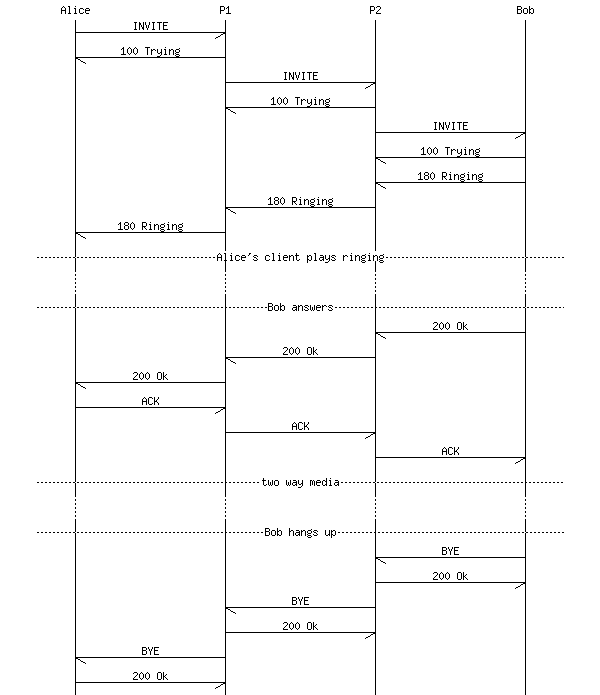
\includegraphics[width=150mm]{./images/msg.png}\\
\caption{Figure showing Message Sequence Chart}
\end{figure}

\chapter{DroidRacer}
\par DROIDRACER provides  a  framework  that generates UI events to systematically test an Android application.It runs unmodified binaries on an instrumented Dalvik VM and in-strumented
Android libraries. A run of the application produces an execution trace, which is analyzed offline for data races by computing the happens-before relation. The control flow between 
different procedures of an Android application is managed to a large extent by  the  Android  runtime  through  callbacks.  DROIDRACER uses  a model of the Android runtime environment to reduce false positives
that would be reported otherwise. Further, DROIDRACER assists in debugging the data races by classifying them based on criteria such as whether one involves multiple threads posting to the same thread
or two co-enabled events executing in an interleaved manner.\\
\section{Modelling the runtime environment}
\par While we do not explicitly model ActivityManagerService (running in the system process) in  the  execution  trace,  we  capture  its  effects  through  the enable
operations on callback procedures. This helps us identify the ordering constraints for lifecycle callbacks made by the Android environment.Through enable operations,we also 
capture the ordering between operations in the trace and UI callbacks.The user action results in the activity being removed from the screen (but not garbage-collected), and 
ActivityManagerService posts a call to the onDestroy callback. This callback executes next writes into the field isActivityDestroyed. Due to the happens-before ordering between
enable and post and post and begin there is a happens-before edge between the write operations 7 and 21 and they do not constitute a data race. Without the enable operation, 
which specifies the environment restriction that onDestroy can only be called after LAUNCH\_ACTIVITY finishes, we could not have derived the required happens-before ordering between 
operations 7 and 21 , resulting in a false positive.\\
\begin{figure}
 \centering
 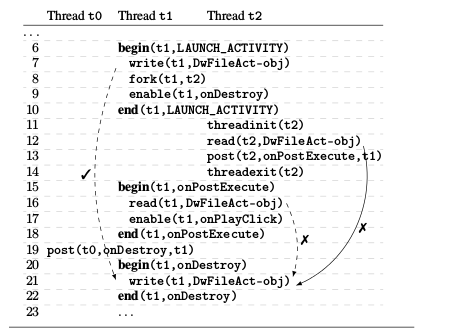
\includegraphics[width=150mm]{./images/partial_execution_trace.png}\\
\caption{Partial exection trace for the scenario in which user clicks the BACK button instead of PLAY button}
\end{figure}
\section{Analysis for data races}
\par Again, we consider the trace in Figure 4.1 The callback onDestroy is  enabled  while  thread t2 is  running  and  if  fired,  it executes on thread t1. Thus, the read and
write operations 12 and 21 may happen in parallel giving rise to a potential data race.

\chapter{Idea and Approach}
\par We are using the droidracer traces to analyze information misuse in android apps.
We try to convert traces obtained from DroidRacer into message sequence chart. For that we follows the following steps:\\
\begin{description}
 \item[$\bullet$Separation] We separate out  stack traces on the basis of tid's or thread ids and rename as like parent\_child.txt file. 
We found out different events from log files an dfound out there are number of events ( such as: ADD\_IDLE\_HANDLER, ENABLE\_LIFECTCLE,ENABLE\_WINDOW-FOCUS,INSTANCE-INTENT,QUEUE\_IDLE,
REMOVE\_IDLE\_HANDLER etc. ) which are not of our corns beacuse they doesn't cause any misuse of objects as given in figure Sheet1 in excel sheet. \\
\begin{figure}
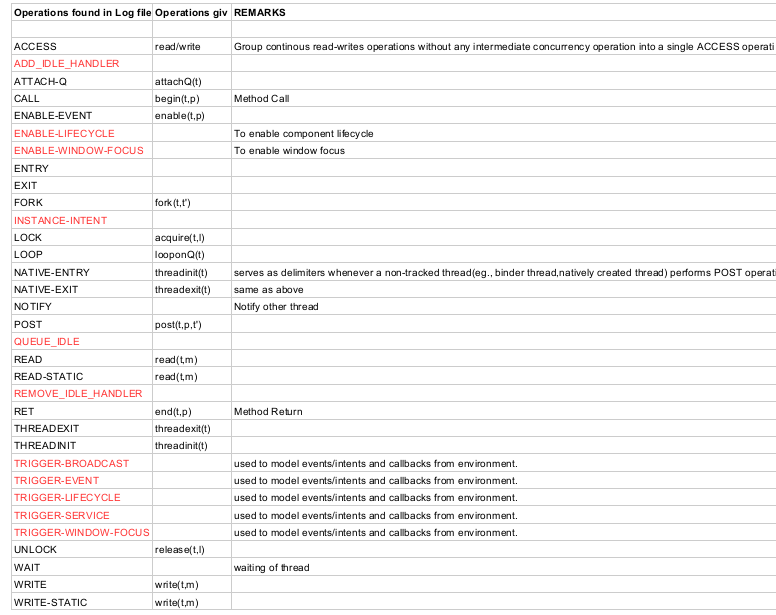
\includegraphics[width=150mm]{./images/sheet-1.png}\\
\caption{All event found in trace file}
\end{figure}
\item[$\bullet$Removal of Unnecessary Events] We remove all these non concerned events from our event set and map it to the operations given in droid racer paper. After that we label different objects and thread under
these operations (Sheet2 in excel sheets).\\
\begin{figure}
\centering
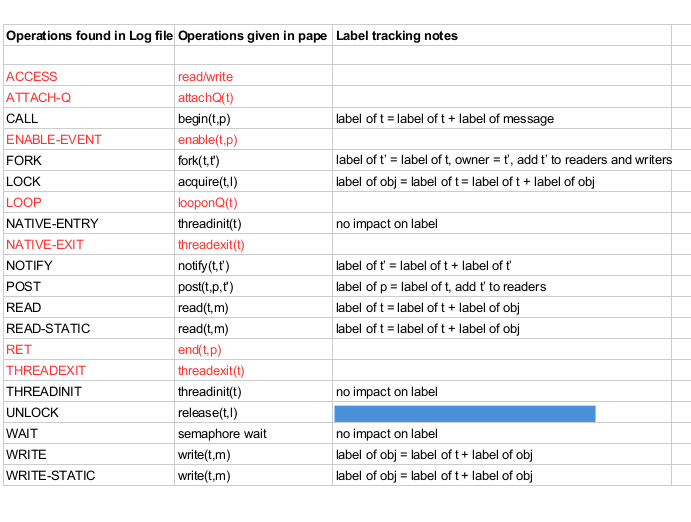
\includegraphics[width=150mm]{./images/sheet-2.png}\\
\caption{Necessary Events for Analysis}  
\end{figure}
\item[$\bullet$Parsing] Parsed each file starting from 1.txt because thread 1 is the main thread in the following ways:\\
\textbf{READ} Read instructions in the trace file:\\
$$ rwId:1 READ tid:1 obj:0x411253f8 class:Ljava/lang/StringBuilder; field:16$$ can be changed into $$READ(1) $$ given that we map obj:0x411253f8 field:16 into some integer id.\\
\textbf{WRITE} Write instructions in trace file:\\
$$ rwId:5 WRITE tid:1 obj:0x411253f8 class:Ljava/lang/StringBuilder; field:16$$  can be changed into $$ WRITE(1)$$ given that we map obj:0x411253f8 field:16 into some integer id.\\
\textbf{FORK} Fork instructions in trace file:
$$ 30 FORK par-tid:1	 child-tid:6$$ can be change into $$ FORK----------------------------------------\textgreater THREADINIT $$ such that arrow from tid:1 pointed to tid:6.Thread id's are already 
arranged at the start of the file. Then both the parent and child id's read their own files one by one.\\
\textbf{WAIT/NOTIFY} WAIT and NOTIFY instructions in stack trace file can be given as:\\
$ WAIT tid:1/
NOTIFY tid:6 notifiedTid:1 $
So if the any file contains WAIT call then we have to wait for other file NOTIFY instruction such that it notifies the thread that is waiting on that for the later thread.Therefore,
it can be changed into:\\
$$ WAIT\textless--------------------------------------------------------NOTIFY $$means some thread(n+i) notifies thread(n).\\
\textbf{LOCK/UNLOCK} LOCK/UNLOCK instructions in trace file:
$$41 LOCK tid:1	 lock-obj:0x41128b90/
48 UNLOCK tid:1	 lock-obj:0x4105e8d0 $$
Lock/Unlock instructions used for synchronisation puroposes can be written as LOCK(2) / UNLOCK(2) givent that lock-obj can be mapped to some integer.\\
\textbf{POST/CALL} POST/CALL instructions in trace file:\\
$$54 POST src:2 msg:6 dest:-1 delay:0/
162 CALL tid:1	 msg:3 $$
So if the any file contains POST call then we have to wait for other file CALL instruction such that it notifies the thread that is waiting on that for the later thread.
$$ POST(13)------------------------------------------------------------------------------------------------\textgreater CALL(13) $$ means some thread(n) post call to some thread(n+i) giving some object
which mapped to 13 integer internally.\\

\item[$\bullet$Merging] Merged two consecutive same event (READ/WRITE) on the same object into one event(READ/WRITE).\\
\item[$\bullet$Labelling]  Labelled out the resultant file obtained after merging and check out any misuse using the rules given by RWFM above.\\

\chapter{Experimentation and Output}
\par We chose twitter application traces for examination.Here are the screenshots of different files given below:\\
Trace file from DroidRacer:\\
\begin{figure}
\centering
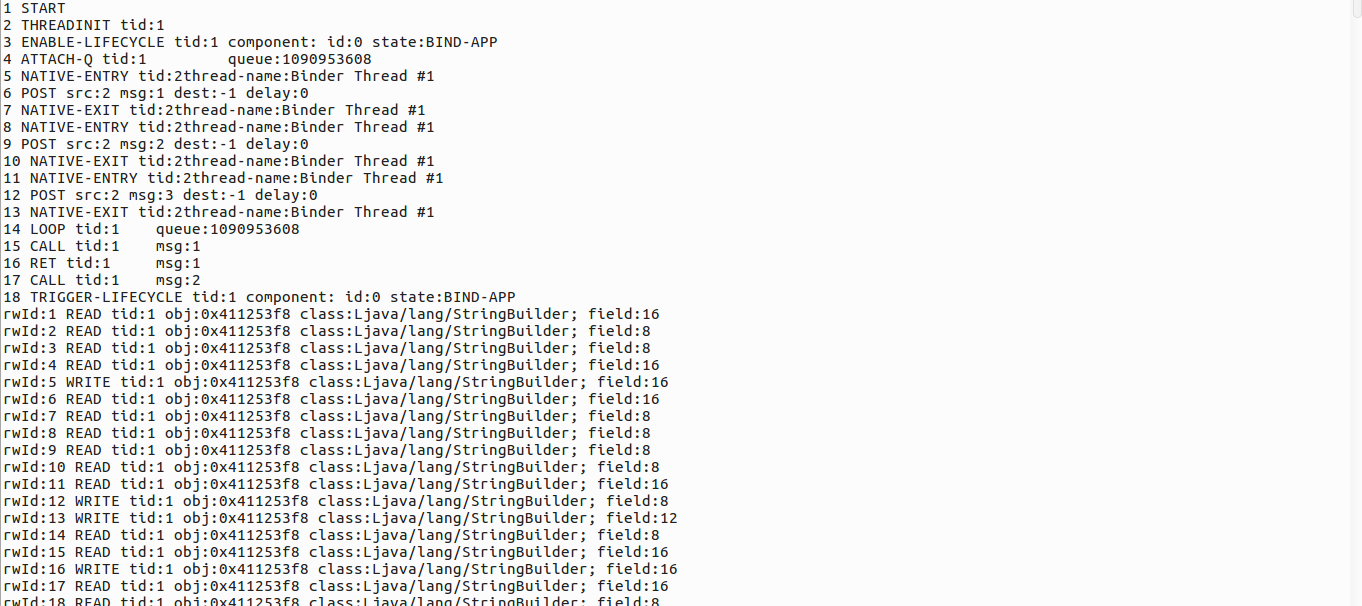
\includegraphics[width=150mm]{./images/traces.png}\\
\caption{Trace File from DroidRacer}
\end{figure}

Message Sequence Chart:\\
\begin{figure}
\centering
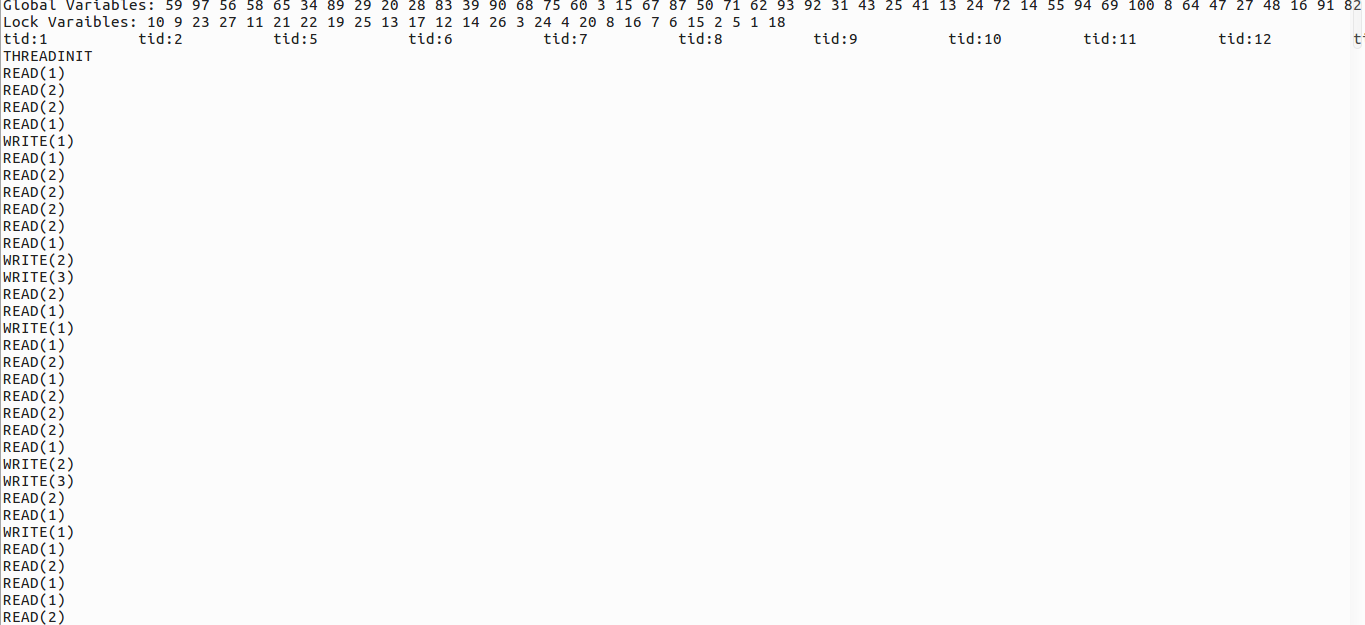
\includegraphics[width=150mm]{./images/msg-traces.png}\\
\caption{Message Sequence Chart for Twitter app trace}
\end{figure}
After Similar Call Merging:\\
\begin{figure}
\centering
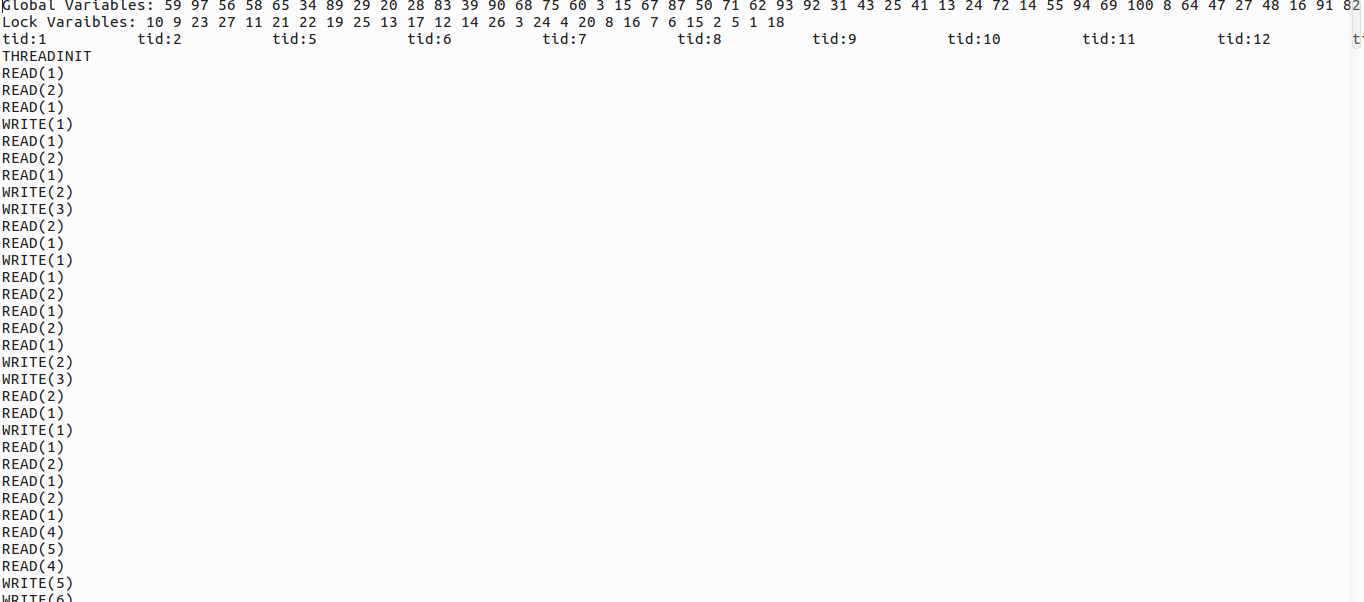
\includegraphics[width=150mm]{./images/merged.png}\\
\caption{Merged File}
\end{figure}
Resultant File with labelling:\\
\begin{figure}
\centering
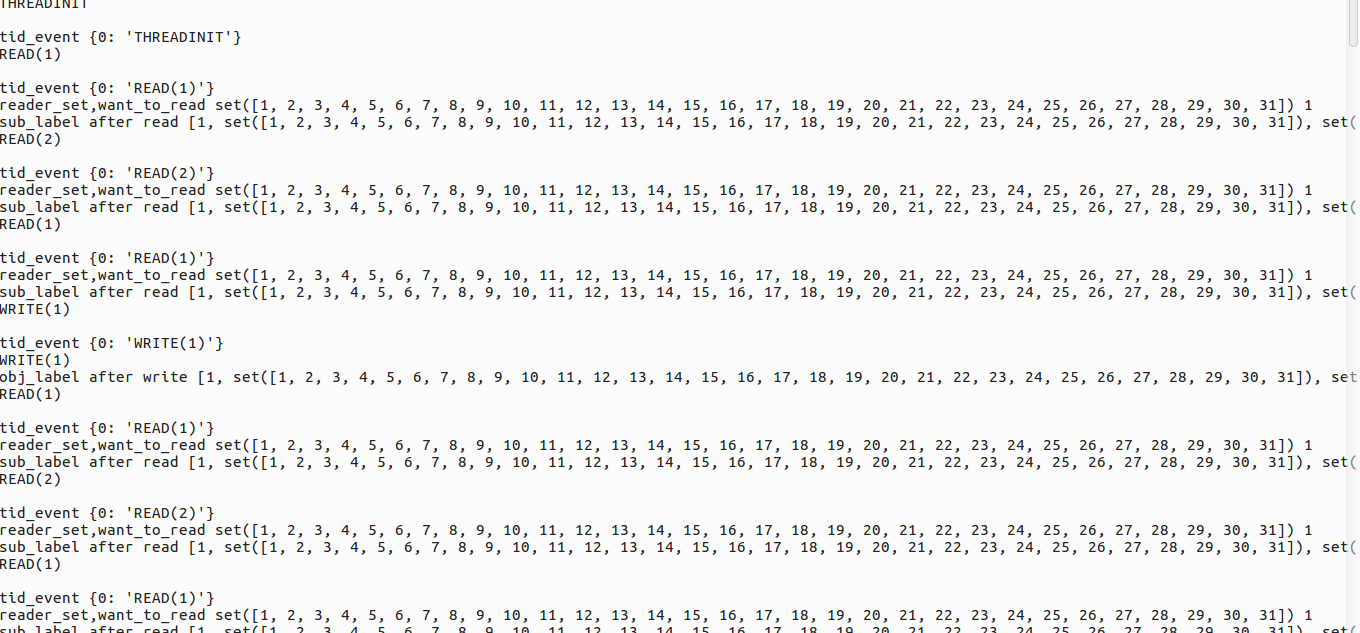
\includegraphics[width=150mm]{./images/output.png}\\
\caption{Labelled file}
\end{figure}
\textbf{OUTPUT}\\
\par There are some scenarios are there such that there is data race in DroidRacer traces and no misuse occurs by using our RWFM model.\\

\end{description}

\chapter{Future Work}
\begin{itemize}
 \item Checking all the possible combination of RWFM on a parallel.
 \item Comparing the result of DroidRacer with RWFM misuse.
\end{itemize}




\end{document}